\documentclass[a4paper,28pt]{report}
\usepackage[top=1in, bottom=1.25in, right=1in, left=1.5in]{geometry}
\usepackage[parfill]{parskip}
\usepackage{setspace}
\usepackage{sectsty}
\chapterfont{\centering\textbf}
\sectionfont{\underline\textbf} %\centering}
\subsectionfont{\underline\textbf}
\usepackage{listings}
\usepackage{titlesec}
\usepackage{fancyhdr}
\renewcommand{\chaptername}{Experiment}
\usepackage{graphicx}
\graphicspath{{}}
\usepackage{multirow}
%
%
%
% % % % % % % % % % % % % % %
\title{
	{CHI Lab Record}\\
	{\large Department of Computer Science and Engineering}\\
	{ College of Engineering Trivandrum}
}
\author{Sandeep Sukumaran}


% % % % % % % % % % % % % % % 
%
%
\begin{document}
\titlespacing*{\section}{0pt}{0.5ex}{.25ex}
%
%
% % % % % % % % % % % % % % % % %
\maketitle
  \begin{titlepage}
  	\begin{center}
  		\vspace*{30pt}
	  	\huge{ COLLEGE OF ENGINEERING TRIVANDRUM}\\
	  	\vspace*{10pt}
		
\includegraphics{Cet_emblem}\\
		\vspace*{20pt}
		\textsc{\Large{\textbf{ CHI LABORATORY RECORD}}}
		%\line(1,0){300}
  	\end{center}
  	\vspace*{20pt}
  	\textsc{	
	  	\\University Reg. No. : 12400048\\
		Name: Sandeep Sukumaran\\
	  	Roll No: 51\\
	  	Class : S7 R\\
	  	From page no. 1 to page no. 52\\\\\\\\\\
		\hspace*{55pt}\textbf{CERTIFIED BONAFIDE RECORD OF WORK DONE BY}\\
		\centerline{\textbf{Sandeep Sukumaran}}
		\\\\\\\\
	  }
	 
	\begin{minipage}[t]{8cm}
		\flushleft
		Thiruvananthapuram
	\end{minipage}
	\hfill
	\begin{minipage}[t]{7cm}
		\flushright
		Staff in charge\\
		Vipin Vasu A.V\\
		Assisstant Professor\\
		Department of CSE
	\end{minipage}

  	
  \end{titlepage}

% % % % % % % % % % % % % % % % %
%
%
\pagenumbering{roman}
\pagestyle{empty}
\tableofcontents
\cleardoublepage
\pagestyle{plain}
\pagenumbering{arabic}
%\input lab_record.toc
%\thispagestyle{empty}
%\chapter{Introduction}
\chapter{Familiarization of components}
%
%
%
\section*{AIM:}
	Familiarization of the components / Cards inside a computer, standard connectors, cords, different ports,
	and various computer peripherals
	
\section*{COMPUTER COMPONENTS:}
\subsection*{MOTHERBOARD}
	The motherboard is the main component inside the case. It is a large rectangular board with integrated circuitry
	that connects the other parts of the computer including the CPU, the RAM, the disk drives as well as any peripherals 	connected via the ports or the expansion slots.
\subsection*{PROCESSOR}
	A central processing unit (CPU), also referred to as a central processor unit,
	[1] is the hardware within
	a computer that carries out the instructions of a computer program by performing the basic arithmetical, logical,
	and input/output operations of the system. A computer can have more than one CPU; this is
	called multiprocessing. Two typical components of a CPU are the arithmetic logic unit (ALU), which
	performs arithmetic and logical operations, and the control unit (CU), which extracts instructions
	from memory and decodes and executes them, calling on the ALU when necessary.
\subsection*{CHIPSET}
	A chipset is a set of electronic components in an integrated circuit that manage the data flow between the
	processor, memory and peripherals. It is usually found in the motherboard of a computer. Because it controls 			communications between the
	processor and external devices, the chipset plays a crucial role in determining system performance. Based
	on Intel Pentium-class microprocessors, the term chipset often refers to a specific pair of chips on the
	motherboard: the northbridge and the southbridge. The northbridge links the CPU to very high-speed devices,
	especially RAM and graphics controllers, and the southbridge connects to lower-speed peripheral buses (such
	as PCI or ISA). 
\subsection*{READ ONLY MEMORY}
	Read-only memory (ROM) is a class of storage medium used in computers and other electronic devices. Data
	stored in ROM cannot be modified, or can be modified only slowly or with difficulty, so it is mainly used to
	distribute firmware (software that is very closely tied to specific hardware and unlikely to need frequent
	updates). Other types of non-volatile memory such as erasable programmable read only memory (EPROM)
	and electrically erasable programmable read-only memory (EEPROM or Flash ROM) are sometimes referred to,
	in an abbreviated way, as "read-only memory" (ROM); although these types of memory can be erased and reprogrammed
	multiple times, writing to this memory takes longer and may require different procedures than
	reading the memory.
\subsection*{BIOS}
	In IBM PC compatible computers, the Basic Input/Output System (BIOS), also known as the system
	BIOS or ROM BIOS, is a de facto standard defining a firmware interface. The fundamental purposes of the
	BIOS are to initialize and test the system hardware components, and to load a bootloader or an operating
	system from a mass memory device. The BIOS additionally provides abstraction layer for the hardware, i.e. a
	consistent way for application programs and operating systems to interact with the keyboard, display, and other
	input/output devices. Variations in the system hardware are hidden by the BIOS from programs that use BIOS
	services instead of directly accessing the hardware.
\subsection*{BUSES}
	Buses connect the CPU to various internal components and to expansion cards for graphics and sound. It is a
	physical arrangement that provides the same logical functionality as a parallel electrical bus.\newline
	The various Bus architectures currently include:
\subsubsection*{PCI Express}
 	PCI Express (Peripheral Component Interconnect Express), officially abbreviated as PCIe, is
	 a high-speed serial computer expansion bus standard designed to replace the older PCI, PCI-X,
	 and AGP bus standards. PCIe has higher maximum system bus throughput, lower I/O pin count and smaller physical 		footprint,
	 better performance-scaling for bus devices, a more detailed error detection and reporting mechanism
	 (Advanced Error Reporting (AER)), and native hot-plug functionality.
\subsubsection*{PCI}
	  PCI, is a local computer bus for attaching hardware devices in a computer. The PCI bus supports the
	  functions found on a processor bus, but in a standardized format that is independent of any particular
	  processor. Devices connected to the bus appear to the processor to be connected directly to the processor
	  bus, and are assigned addresses in the processor's address space. Typical PCI cards used in PCs include: network 			cards, sound
	  cards, modems, extra ports such as USB or serial, TV tuner cards and disk controllers.
\subsubsection*{SATA}
	   Serial ATA (Advance Technology Attachment)(SATA) is a computer bus interface that
	   connects host bus adapters to mass storage devices such as hard disk drives and optical drives. Serial ATA
	   replaces the older AT Attachment standard (ATA later referred to as Parallel ATA or PATA), offering
	   several advantages over the older interface: reduced cable size and cost (seven conductors instead of 40),
	   native hot swapping, faster data transfer through higher signalling rates, and more efficient transfer through
	   an (optional) I/O queuing protocol.
\subsection*{PORTS}
	   A port serves as an interface between the computer and other computers or peripheral devices. Ports are classified 		as either serial ports or parallel ports
	   based on the mode of data transfer. Hot-swappable ports can be connected while equipment is running. Plug-and-play 		ports are designed so that the connected
	   devices automatically start handshaking as soon as the hot-swapping is done. USB ports and FireWire ports are
	   plug-and-play.The most commonly used ports in a computer are:
\subsubsection*{SERIAL PORT}
	    In computing, a serial port is a serial communication physical interface through which
	    information transfers in or out one bit at a time (in contrast to a parallel port).Throughout most of the
	    history of personal computers, data was transferred through serial ports to devices such as modems,
	    terminals and various peripherals.The common applications for the serial port include
	    dial up modems, GPS receivers, Bar code scanners, Serial mouse etc.
\subsubsection*{PARALLEL PORT}
	 A parallel port is a type of interface found on computers(personal and otherwise) for
	connecting peripherals. In computing, a parallel port is a parallel communication physical interface. It is
	also known as a printer port or Centronics port. The parallel port is usually implemented using a 25 pin DB-25 connector.
\subsubsection*{ USB}
	 Universal Serial Bus (USB) is an industry standard developed in the mid-1990s that defines the
	cables, connectors and communications protocols used in a bus for connection, communication, and power
	supply between computers and electronic devices. USB was designed to standardize the connection
	of computer peripherals (including keyboards, pointing devices, digital cameras, printers, portable media
	players, disk drives and network adapters) to personal computers, both to communicate and to
	supply electric power. USB has effectively replaced a variety of earlier interfaces, such as serial and parallel 		ports,
	as well as separate power chargers for portable devices. The presently used USB standard is USB 3.0 which
	has a data rate of upto 5 GB/sec.
\subsubsection*{ SCSI}
	 Small Computer System Interface(SCSI) is a set of standards for physically connecting and
	transferring data between computers and peripheral devices. The SCSI standards define commands,
	protocols and electrical and optical interfaces. SCSI is most commonly used for hard disks and tape drives,
	but it can connect a wide range of other devices, including scanners and CD drives, although not all
	controllers can handle all devices. SCSI is an intelligent, peripheral, buffered, peer to peer interface. It hides
	the complexity of physical format. Every device attaches to the SCSI bus in a similar manner. Up to 8 or 16
	devices can be attached to a single bus. There can be any number of hosts and peripheral devices but there
	should be at least one host.
\subsubsection*{ESATA}
	 Standardized in 2004, eSATA (\emph{external} SATA) provides a variant of SATA meant for
	external connectivity. It uses a more robust connector, longer shielded cables, and stricter (but backwardcompatible)
	electrical standards.
\subsubsection*{FIREWIRE}
	 Firewire (IEEE 1394) is a serial bus interface standard for high-speed communications
	and isochronous real-time data transfer.The system is commonly used to connect data storage
	devices and DV (digital video) cameras, but is also popular in industrial systems for machine vision and
	professional audio systems. It is preferred over the more common USB for its greater effective speed and
	power distribution capabilities. Firewire supports data transfer rates of up to 3200 Mbits/sec.
\subsection*{EXPANSION DEVICES}
	The expansion card (also expansion board, adapter card or accessory card) is a printed circuit board that can
	be inserted into an electrical connector, or expansion slot on a computer motherboard, backplane or riser card to
	add functionality to computer system via the expansion bus. The primary purpose of an expansion card is to
	provide or expand on features not offered by the motherboard. Some commonly used expansion cards are:
\subsubsection*{VIDEO CARD} 
	A video card is an expansion card which generates a feed of output images to a display.
	Most video cards offer various functions such as accelerated rendering of 3D scenes and 2D graphics,
	MPEG-2/MPEG-4 decoding, TV output, or the ability to connect multiple monitors (multi-monitor). It is
	also called a video controller or graphics controller.
\subsubsection*{SOUND CARD}
	 A sound card (also known as an audio card) is an internal computer expansion card that
	facilitates the input and output of audio signals to and from a computer under control of computer
	programs. Typical uses of sound cards include providing the audio component for multimedia applications
	such as music composition, editing video or audio, presentation, education and entertainment (games) and
	video projection.
\subsubsection*{ NETWORK INTERFACE CONTROLLER CARD}
	 A network interface controller (NIC) is a computer hardware component
	that connects a computer to a computer network. The network controller implements the electronic circuitry
	required to communicate using a specific physical layer and data link layer standard such as Ethernet, WiFi
	or Token Ring.
\subsubsection*{TV TUNER CARD}
	 A TV tuner card is a kind of television tuner that allows television signals to be received by
	a computer. Most TV tuners also function as video capturecards, allowing them to record television
	programs onto a hard disk much like the digital video recorder (DVR) does.
\subsection*{SECONDARY STORAGE DEVICES}
	Computer data storage, often called storage or memory, is a technology consisting of computer components
	and recording media used to retain digital data. It is a core function and fundamental components of
	computers. In practice, almost all computers use a storage hierarchy, which puts fast but expensive and volatile
	small storage options close to the CPU and slower but larger, permanent and cheaper options farther away. The
	permanent storage is usually referred to as secondary storage. Secondary storage devices can be broadly
	classified into two:
\subsubsection*{FIXED MEDIA}
	\paragraph{HARD DISK DRIVES}
	  Hard drive, hard disk, or disk drive is a device for
	storing and retrieving digital information, primarily computer data. It consists of one or more rigid rapidly rotating discs (often referred to as platters), coated with magnetic material and
	with magnetic heads arranged to write data to the surfaces and read it from them. An HDD retains its
	data even when powered off. Data is read in a random-access manner. HDDs are
	connected to systems by standard interface cables such as SATA (Serial ATA), USB or SAS (Serial
	attached SCSI) cables. The capacity of modern hard drives ranges from 500 GB to 4 TB.
	\paragraph{SOLID STATE DRIVES}
	A solid-state drive (SSD), sometimes called a solid-state disk or electronic disk, is a
	data storage device that uses solid-state memory to store persistent data with the intention of providing
	access in the same manner of a traditional block I/O hard disk drive. SSDs are distinguished from
	traditional magnetic disks such as hard disk drives (HDDs) or floppy disk, which are electromechanical
	devices containing spinning disks and movable read/write heads. Compared with electromechanical
	disks, SSDs are typically more resistant to physical shock, run more quietly, have lower access time,
	and less latency. The capacity of modern
	SSDs usually ranges from 64 GB to 1 TB.
\subsubsection*{REMOVABLE MEDIA}
	\paragraph{OPTICAL DISK DRIVES}
	 An optical disc drive (ODD) is a disk drive that uses laser light or electromagnetic
	waves within or near the visible light spectrum as part of the process of reading or writing data to or
	from optical discs. Some drives can only read from discs, but recent drives are commonly both readers
	and recorders, also called burners or writers. Compact discs, DVDs, and Blu-ray discs are common
	types of optical media which can be read and recorded by such drives.
	\paragraph{FLOPPY DISK DRIVES} 
	They are used for reading and writing to floppy disks, an outdated storage media
	consisting of a thin disk of a flexible magnetic storage medium. These were once standard on most
	computers but are no longer in common use. Floppy disks, initially as 8-inch (200 mm) media and later
	in 5.25-inch (133 mm) and 3.5-inch (90 mm) sizes, were a ubiquitous form of data storage and
	exchange from the mid-1970s well into the first decade of the 21st century. Floppies are used today
	mainly for loading device drivers not included with an operating system release.
	\paragraph{USB Flash drives}
	 A USB flash drive is a data storage device that includes flash memory with an
	integrated Universal Serial Bus (USB) interface. USB flash drives are typically removable and
	rewritable, and physically much smaller than an optical disc. Modern USB drives can store data up to
	256 GB.
	\paragraph{TAPE DRIVES}
	 A tape drive is a data storage device that reads and writes data on a magnetic
	tape. Magnetic tape data storage is typically used for offline, archival data storage. Tape media
	generally has a favorable unit cost and long archival stability. A tape drive provides sequential
	access storage, unlike a disk drive, which provides random access storage. A disk drive can move to
	any position on the disk in a few milliseconds, but a tape drive must physically wind tape between reels
	to read any one particular piece of data. As a result, tape drives have very slow average seek times.
	However, the storage capacity of magnetic tapes is considerably more than other secondary storage
	mediums.
\subsection*{INPUT AND OUTPUT PERIPHERALS}
	Input and output devices are typically housed externally to the main computer chassis. The following are either
	standard or very common to many computer systems.
\subsubsection*{INPUT DEVICES}
	\paragraph{KEYBOARDS}
		 A keyboard is a device to input text and characters by depressing buttons. It is a typewriterstyle
	device, which uses an arrangement of buttons or keys, to act as mechanical levers or electronic
	switches. While most keyboard keys produce letters, numbers or signs (characters), other keys or
	simultaneous key presses can produce actions or execute computer commands.
	\paragraph{MOUSE}
	 A mouse is a pointing device that functions by detecting two-dimensional motion relative to its
	supporting surface. Physically, a mouse consists of an object held under one of the user's hands, with
	one or more buttons. The mouse's motion typically translates into the motion of a pointer on a display,
	which allows for fine control of a graphical user interface. 
	\paragraph{TRACKBALL}
	 A trackball is a pointing device consisting of a ball held by a socket containing sensors to
	detect a rotation of the ball about two axes—like an upside-down mouse with an exposed protruding
	ball. The user rolls the ball with the thumb, fingers, or the palm of the hand to move a pointer.
	\paragraph{TOUCHSCREEN}
	 A touchscreen is an electronic visual display that the user can control through simple
	or multi-touch gestures by touching the screen with one or more fingers. Some touchscreens can also
	detect objects such as a stylus or ordinary or specially coated gloves. The user can use the touchscreen
	to react to what is displayed and to control how it is displayed (for example by zooming the text size).
		The touchscreen enables the user to interact directly with what is displayed, rather than using
	a mouse, touchpad, or any other intermediate device. 
	\paragraph{JOYSTICK}
	 A joystick is an input device consisting of a stick that pivots on a base and reports its angle or
	direction to the device it is controlling. Joysticks are often used to control video games, and usually
	have one or more push-buttons whose state can also be read by the computer.
	\paragraph{IMAGE SCANNER}
	 In computing, an image scanner, often abbreviated to just scanner is a device that
	optically scans images, printed text, handwriting, or an object, and converts it to a digital image.
	Common examples found in offices are variations of the desktop (or flatbed) scanner where the
	document is placed on a glass window for scanning. Hand-held scanners, where the device is moved by
		hand, have evolved from text scanning "wands" to 3D scanners used for industrial design, reverse
	engineering, test and measurement, orthotics, gaming and other applications. Mechanically driven
	scanners that move the document are typically used for large-format documents, where a flatbed design
	would be impractical. Modern scanners typically use a charge-coupled device(CCD) or a Contact
	Image Sensor(CIS) as the image sensor, whereas older drum scanners use a photomultiplier tube as the
	image sensor. A rotary scanner, used for high-speed document scanning, is another type of drum
	scanner, using a CCD array instead of a photomultiplier. Other types of scanners are planetary
	scanners, which take photographs of books and documents, and 3D scanners, for producing three dimensional
	models of objects.
	\paragraph{MICROPHONE} 
	A microphone is an acoustic to electric transducer or sensor that converts sound into an
	electrical signal. Microphones are used to input audio data into the computer for processing.
\subsubsection*{OUTPUT DEVICES}
		\paragraph{PRINTERS}
	 In computing, a printer is a peripheral which produces a representation of an electronic
	document on physical media such as paper or transparency film. Many printers are local peripherals
	connected directly to a nearby personal computer. Individual printers are often designed to support both
	local and network connected users at the same time. Depending on the technology used, there can be
	several variants of printers such as inkjet printers, laser printers, dot matrix printers, thermal printers
	etc.
	\paragraph{COMPUTER MONITORS}
	 A monitor or a display is an electronic visual display for computers. The monitor
	comprises the display device, circuitry and an enclosure. The display device in modern monitors is
	typically a thin film transistor liquid crystal display(TFT-LCD) thin panel, while older monitors use
	a cathode ray tube(CRT) about as deep as the screen size.
	\paragraph{SPEAKERS}
	 Computer speakers, or multimedia speakers, are speakers external to a computer, that disable
	the lower fidelity built-in speaker. They often have a low-power internal amplifier. The standard audio
	connection is a 3.5 mm (approximately 1/8 inch) stereo phone connector often color-coded lime green
	(following the PC 99 standard) for computer sound cards. Analog A/V connectors often use shielded cables to
	inhibit radio frequency interference(RFI) and noise. Some commonly used connectors are as follows:
	 \paragraph{RCA}
	  An RCA connector, sometimes called a phono connector or cinch connector, is a type of electrical
	connector commonly used to carry audio and video signals. The connectors are also sometimes casually
	referred to as A/V jacks.
	\paragraph{VGA}
	 A Video Graphics Array(VGA) connector is a three-row 15-pin DE-15 connector which carries
	video signals. The 15-pin VGA connector is found on many video cards, computer monitors, and high
	definition television sets.
	\paragraph{DVI}
	 Digital Visual Interface(DVI) is a video display interface developed by the Digital Display Working
	Group(DDWG). The digital interface is used to connect a video source to a display device, such as
	a computer monitor.
	\paragraph{HDMI}
	 HDMI (High-Definition Multimedia Interface) is a compact audio/video interface for
	transferring uncompressed video data and compressed/uncompressed digital audio data from a HDMI compliant
	device ("the source device") to a compatible computer monitor, video projector, digital
	television, or digital audio device.

%
%
%
\chapter{Assembly of computer}
%
%
%
%
\section*{AIM:}
To study the assembly of a computer from its components
\section*{PROCEDURE:}
Following are the steps involved in assembling a computer from its components:

\textbf{\underline{Step 1}:} Open the case by removing the side panels.


\textbf{\underline{Step 2}:} Install the Power Supply.

\hspace{40pt}Power supply installation steps include the following:

\hspace{40pt}Insert the power supply into the case.

\hspace{40pt}Align the holes in the power supply with the holes in the case.

\hspace{40pt}Secure the power supply to the case using the proper screws.


\textbf{\underline{Step 3}:} Attach Components to the Motherboard

\hspace{40pt}\textbf{i)} CPU on Motherboard

\hspace{50pt}The CPU and motherboard are sensitive to electrostatic discharge.
\newline
\hspace*{50pt}The CPU is secured to the socket on the motherboard with a locking assembly.
\\\hspace*{50pt}Thermal compound is applied to help keep the CPU cool.

\hspace{40pt}\textbf{ii)} Heat Sink/Fan Assembly

\hspace{50pt}  The Heat Sink/Fan Assembly is a two-part cooling device.
\\\hspace*{50pt}  The heat sink draws heat away from the CPU.

\hspace{40pt}\textbf{iii)} Install RAM

\hspace{50pt}  RAM provides temporary data storage for the CPU and should be installed in the\\\hspace*{50pt}  motherboard before the motherboard is placed in the computer case.

\hspace{40pt}\textbf{iv)} Install motherboard in the computer case.


\textbf{\underline{Step 4}:} Install the Hard Disk drive in the 3.5 inch internal drive bay using screws.


\textbf{\underline{Step 5}:} Install optical disc drive and floppy disc drive in the external drive bays provided for\\\hspace*{40pt}the same.


\textbf{\underline{Step 6}:} Install Adapter cards: Expansion cards such as NIC cards, video cards, sound cards\\\hspace*{40pt}etc. should be installed in the slots (PCI, PCIe) provided for the same in the mother-\\\hspace*{40pt}board.


\textbf{\underline{Step 7}:} Connect all the internal power and data cables. Power cables distribute electricity \\\hspace*{40pt}from the power supply to the motherboard and other components. Data cables\\\hspace*{40pt}transmit data between the motherboard and storage devices, such as hard drives.


\textbf{\underline{Step 8}:} Close the case by reattaching the side panels. Connect the external cables.


\textbf{\underline{Step 9}:} Boot computer for first time. The BIOS will perform a Power On Self Test (POST) to\\\hspace*{40pt}check all of the internal components. If a device is malfunctioning, an error or beep\\\hspace*{40pt}code will be generated.


\textbf{\underline{Step 10}:} If the computer is functioning properly, install a suitable operating system.

\section*{RESULT:}
The computer components have been studied and assembled into a working computer.
%
%
%
%
%
%\chapter{Serial Port Experiments}

\chapter{COM Port base address}
%
%
\section*{AIM:}
To find the base address of the COM port in a system.
\section*{THEORY:}
COM is the original, yet still common, name of the serial port interface on IBM-PC compatible computers. It might refer not only to physical ports, but also to virtual ports, such as ports created by Bluetooth or USB-to-serial adapters. COM ports are usually associated with 4 memory addresses as shown below:

\begin{center}
\bgroup
\def\arraystretch{1.5}
\begin{tabular}{ |c|c|c| }
\hline
\textbf{NAME} & \textbf{ADDRESS} & \textbf{IRQ}\\
\hline
COM1 & 0x3f8 & 4\\
\hline
COM2 & 0x2f8 & 3\\
\hline
COM3 & 0x3e8 & 4\\
\hline
COM4 & 0x2e8 & 3\\
\hline
\end{tabular}
\egroup
\end{center}

The base addresses for the COM ports can be read from the BIOS data area. The addresses in the BIOS data
area that store the COM port base addresses are as follows:

\begin{center}
\bgroup
\def\arraystretch{1.5}
\begin{tabular}{ |c|c| }
\hline
\textbf{Start Address} & \textbf{Function}\\
\hline
0000:0400 & COM1's Base Address\\
\hline
0000:0402 & COM2's Base Address\\
\hline
0000:0403 & COM3's Base Address\\
\hline
0000:0404 & COM4's Base Address\\
\hline
\end{tabular}
\egroup
\end{center}

\section*{PROCEDURE:}
Execute the following program to find the base address of the COM port.

\section*{PROGRAM:}
\begin{lstlisting}
#include <stdio.h>
#include <string.h>

int main()
{
     char s[100],string[100];
     int com=0;
     
     //--Executing BASH script to read all messages in kernel ring buffer,
     //  search for the string "ttyS" in these messages and
     //  redirect the search results into a text file for further use
     
     system("dmesg | grep ttyS > out.txt");
     
     FILE *fp;
     fp=fopen("out.txt","r");
     
     while( !feof(fp) )
     {
          fscanf(fp, "%s", string);
          if( strcmp(string,"I/O") == 0 )
          {
               fscanf(fp, "%s", s);
               printf("COM PORT%d ADDRESS IS %s\n",com,s);
          }
     }
     
     fclose(fp);
     return 0;
}
\end{lstlisting}

\section*{RESULT}
The program has been executed and the output verified.
%
%
\chapter{Serial Port Inter-Computer Communication}
%
%
%
\section*{AIM:}To transmit data between two computers using the serial port

\section*{THEORY:}
Devices that use serial cables for their communication are split into two categories: \textbf{DCE} (\emph{Data Communications Equipment}) and \textbf{DTE} (\emph{Data Terminal Equipment}). A modem is a DCE while a computer/terminal is a DTE. Serial ports can be 25 pin or 9 pin ports. A D-type 25 pin or 9 pin male connector is used to connect to the serial port. The pin connections for the serial port connectors are as shown below:

\begin{table}[h]
\centering
%\label{my-label}
\bgroup
\def\arraystretch{1.5}
\begin{tabular}{|c|c|c|c|}
\hline
\textbf{D-Type-25 Pin No.}  & \textbf{D-Type-9 Pin No.}  & \textbf{Abbreviation} & \textbf{Full Name}  \\ \hline
Pin 2 & Pin 3 & TD & Transmit Data \\ \hline
Pin 3 & Pin2  & RD & Receive Data\\ \hline
Pin 4 & Pin 7 & RTS & Request To Send     \\ \hline
Pin 5 & Pin 8 & CTS & Clear To Send       \\ \hline
Pin 6 & Pin 6 & DSR & Data Set Ready      \\ \hline
Pin 7 & Pin 5 & SG & Signal Ground       \\ \hline
Pin 8 & Pin 1 & CD & Carrier Detect      \\ \hline
Pin 20 & Pin 4 & DTR & Data Terminal Ready \\ \hline
Pin 22 & Pin 9 & RI&   Ring Indicator\\ \hline
\end{tabular}
\caption{Serial Port Connector Pin Connections}
\egroup
\end{table}
%
%
%
\newpage
\begin{table}[h]
\centering
%\caption{My caption}
%\label{my-label}
\bgroup
\def\arraystretch{1.5}
\begin{tabular}{|c|c|p{7cm}|}
\hline
\textbf{Abbreviation} & \textbf{Full Name}  & \textbf{Function}\\
\hline
TD & Transmit Data & Serial Data Output (TXD)\\
\hline
RD  & Receive Data & Serial Data Input (RXD) \\
\hline
CTS & Clear To Send & This line indicates that the modem is ready to exchange data \\ \hline
DCD & Data Carrier Detect & When the modem detects a carrier from the modem at the other end of the phone line, this line becomes active \\
\hline
DSR & Data Set Ready & This tells the UART that the modem is ready to establish a link\\                                             \hline
DTR & Data Terminal Ready & This is the opposite of DTR and tells the modem that the UART is ready to link\\
\hline
RTS & Request To Send & This line informs the modem that the UART is ready to exchange data\\
\hline
RI & Ring Indicator & This line goes active when the modem detects a ringing signal from the PTSN\\
\hline
\end{tabular}
\egroup
\end{table}
%

\bgroup
\textbf{\underline{Null Modems}:}
A null modem is used to connect two DTEs together. This is usually used as a cheap way to transfer files between computers. The wiring of a null modem is as shown below:
\begin{figure}[h]
\centering
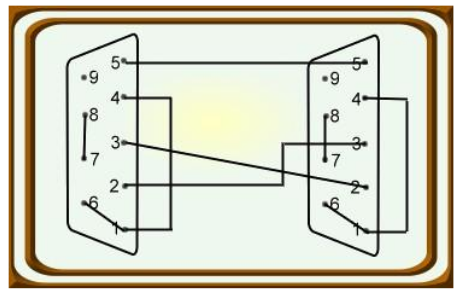
\includegraphics[scale=0.5]{null-modem}
\caption{Wiring of a null modem}
\end{figure}
\egroup

The null modem tricks the computer into thinking that it is talking to a modem and not another computer. Any data transmitted from the first computer must be received by the second and thus TD of the first is connected to
RD of the second. The second computer must have the same setup-thus RD of the first is connected to TD of the second. Signal Ground (SG) must also be connected so both grounds are common. The Data Terminal Ready is looped back to Data Set Ready and Carrier Detect on both computers. When the Data Terminal Ready is asserted active, the Data Set Ready and Carrier Detect immediately become active. At this point the computer thinks the Virtual Modem to which it is connected is ready and has detected the carrier of the other modem. As both computers
communicate at the same speed, flow control is not needed. Thus these two lines are also linked together on each computer. When the computer wishes to send data, it asserts the Request to Send high and, as it is connected to the Clear to Send, it immediately gets a reply that it is ok to send and does so.

\section*{PROCEDURE:}
\textbf{\underline{STEP 1}:} Connect the two computers using Null Modem

\textbf{\underline{STEP 2}:} Enter program at both computers

\textbf{\underline{STEP 3}:} Enter characters at sender side and observe output at receiver side. The computers  \hspace*{48pt}communicate in half duplex, alternating as sender and receiver.

\section*{PROGRAM:}
\begin{lstlisting}
#include <sys/io.h>
#include <stdio.h>
#include <unistd.h>
#define PORT 0x3f8

int serial_received(){ return inb(PORT + 5) & 1;}

char read_serial(){
      while(serial_received() == 0);
      return inb(PORT);
}

int is_transmit_empty(){ return inb(PORT + 5) & 0x20;}

void write_serial(char a){
      while(is_transmit_empty() == 0);
      outb(a,PORT);
}

int main(){

      //--Granting permissions on ports
      
      if( ioperm(PORT,10,1) == -1){
           printf("\nError in granting permissions.\n");
           return -1;
      }else{}
      
      //--Initializng ports
      outb(0x00,PORT+1);
      outb(0x80,PORT+3);
      outb(0x03,PORT);
      outb(0x00,PORT+1);
      outb(0x03,PORT+3);
      outb(0xC0,PORT+2);
      outb(0x0B,PORT+4);
      
      char ch;
      
      //--Infinite loop for half duplex communication follows.
      //--Here,the host waits for data from the peer and then transmits
      //--data input(from the user via keyboard) to the peer.
      //--The peer has the same code with transmission occuring initially.
      
      while(1){
            printf("Waiting to receive\n");
            printf("\nRead the character :%c\n",read_serial());
            printf("\nEnter char to send :");
            scanf(" %c", &ch);
            printf("Sending  %c\n",ch);
            write_serial(ch);
            printf("Sent...\n");
      }
      
      //--Revoking permissions initially granted
      ioperm(PORT,10,0);
      
      return 0;
}
\end{lstlisting}

\section*{RESULT}
The program has been executed and the output verified.
%
%
%
%
\chapter{8051 Serial Communication}
\section*{AIM:}
To transfer 

 1) Single data between 8051 microcontroller ICs.
  
 2) an array of numbers  between 8051 microcontroller ICs.

\section*{ALGORITHM:}
\textbf{Single data transfer}

\large{Sender:}\\

\textbf{\underline{STEP 1}:} Move element to be transfered into SBUF

\vspace*{10pt}
\large{Receiver:}

\textbf{\underline{STEP 1}:} Clear R1 bit 

\textbf{\underline{STEP 2}:} When R1 is set, move SBUF into an external memory location



\section*{PROGRAM:}
\textbf{Sender:}
\begin{lstlisting}
      MOV SBUF ,#FF
LOOP: SJMP LOOP
\end{lstlisting}

\newpage

\textbf{Receiver:}
\begin{lstlisting}
                MOV DPTR,#4500
                CLR 98               ; 98 = RI 
DATA_NOT_READY: JNB R1,DATA_NOT_READY
                MOV A,SBUF
                MOVX @DPTR,A
            EL: SJMP EL
\end{lstlisting}




\section*{Sample Output}
At the receiver side

(4500): FF

\section*{ALGORITHM:}
\textbf{Array transfer}

\large{Sender:}

\textbf{\underline{STEP 1}:} Move count value into register R2

\textbf{\underline{STEP 2}:} Clear RI

\textbf{\underline{STEP 3}:} Move element to be transfered into register A

\textbf{\underline{STEP 4}:} Move contents of register A into SBUF

\textbf{\underline{STEP 5}:} If RI bit is set, decrement R2 and goto step 2

\large{Receiver:}\\

\textbf{\underline{STEP 1}:} Clear RI 

\textbf{\underline{STEP 2}:} If RI bit is set, move content of SBUF into register A

\textbf{\underline{STEP 3}:} Store A in a memory location

\textbf{\underline{STEP 4}:} Move 01 into SBUF

\textbf{\underline{STEP 5}:} Goto step 1

\section*{PROGRAM:}
\textbf{Sender:}
\begin{lstlisting}
           MOV DPTR,#4200
           MOV R2,0A
SEND_LOOP: CLR 98             ; 98 = RI
           MOV A,@DPTR
           MOV SBUF,A
           INC DPTR
     LOOP: JNB 98,LOOP
           DJNZ R2,SEND_LOOP
 END_LOOP: SJMP END_LOOP
\end{lstlisting}

\vspace{20pt}

\textbf{Receiver:}
\begin{lstlisting}
           MOV DPTR,#4500
REC_LOOP:  CLR 98             ; 98 = RI
    LOOP:  JNB 98,LOOP
           MOV A,SBUF
           MOVX @DPTR,A
           INC DPTR
           MOV SBUF,#01
           SJMP REC_LOOP
\end{lstlisting}


\section*{Sample Input}
At the sender side

01 02 03 04 05 06

\section*{Sample Output}
At the receiver side

01 02 03 04 05 06

\section*{RESULT }
The program has been executed and the output verified.
%
%\chapter{Parallel Port Experiments}
\newpage
\chapter{LED Ring Counter}
%
%
%
\section*{AIM:}
To light up LEDs in a ring counter pattern using the parallel port
\section*{THEORY:}
A parallel port is a type of interface found on computers (personal and otherwise) for connecting peripherals. In computing, a parallel port is a parallel communication physical interface. It is also known as a printer port or Centronics port. The port is composed of 4 control lines, 5 status lines and 8 data lines. The connector for the parallel port is a 25 pin D-Type female connector. The parallel port pinout is as shown below:

\begin{figure}[h]
\centering
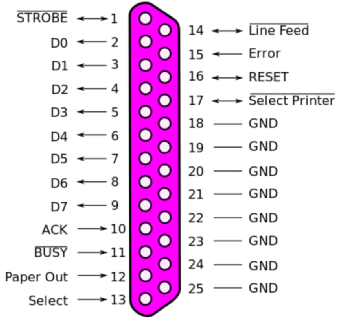
\includegraphics[scale=0.5]{parallel-port-pinout}
\caption{Parallel port pinout}
\end{figure}

The parallel port has three commonly used port addresses as shown below:

\newpage
\begin{table}[h]
\centering
\bgroup
\def\arraystretch{1.5}
\begin{tabular}{ |c|p{7cm}| }
\hline
\textbf{Address} & \textbf{Notes}\\
\hline
3BCh - 3BFh & Used for parallel ports which were incorporated onto Video cards - doesn't support ECP addresses\\
\hline
378h - 37Fh & Usual address for LPT1\\
\hline
278h - 27Fh & Usual address for LPT2\\
\hline
\end{tabular}
\caption{Parallel port base addresses}
\egroup
\end{table}

The parallel port is associated with three software registers namely- the data port, the status port, and the control port.
These ports can be used to read/write data and control the operation of the parallel port. A detailed description of the individual bits in these registers is given below:

\begin{table}[h]
\centering
\bgroup
\def\arraystretch{1.5}
\begin{tabular}{|c|c|c|c|c|}
\hline
\textbf{Offset}           & \textbf{Name}              & \textbf{Read/Write}    & \textbf{Bit No.} & \textbf{Properties} \\ \hline
\multirow{8}{*}{Base + 0} & \multirow{8}{*}{Data Port} & \multirow{8}{*}{Write} & Bit 7            & Data 7              \\ \cline{4-5} 
                          &                            &                        & Bit 6            & Data 6              \\ \cline{4-5} 
                          &                            &                        & Bit 5            & Data 5              \\ \cline{4-5} 
                          &                            &                        & Bit 4            & Data 4              \\ \cline{4-5} 
                          &                            &                        & Bit 3            & Data 3              \\ \cline{4-5} 
                          &                            &                        & Bit 2            & Data 2              \\ \cline{4-5} 
                          &                            &                        & Bit 1            & Data 1              \\ \cline{4-5} 
                          &                            &                        & Bit 0            & Data 0              \\ \hline
\end{tabular}
\caption{Data Port register bits}
\egroup
\end{table}

The data port is simply used for outputting data on the Parallel Port's data lines (Pins 2-9). This register is normally a write only port. However, modern parallel ports are often bi-directional, and data can be read from the data port address.

\begin{table}[h]
\centering
\bgroup
\def\arraystretch{1.5}
\begin{tabular}{|c|c|c|c|c|}
\hline
\textbf{Offset}           & \textbf{Name}                & \textbf{Read/Write}        & \textbf{Bit No.} & \textbf{Properties} \\ \hline
\multirow{8}{*}{Base + 1} & \multirow{8}{*}{Status Port} & \multirow{8}{*}{Read Only} & Bit 7            & Busy                \\ \cline{4-5} 
                          &                              &                            & Bit 6            & Ack                 \\ \cline{4-5} 
                          &                              &                            & Bit 5            & Paper Out           \\ \cline{4-5} 
                          &                              &                            & Bit 4            & Select In           \\ \cline{4-5} 
                          &                              &                            & Bit 3            & Error               \\ \cline{4-5} 
                          &                              &                            & Bit 2            & IRQ                 \\ \cline{4-5} 
                          &                              &                            & Bit 1            & Reserved            \\ \cline{4-5} 
                          &                              &                            & Bit 0            & Reserved              \\ \hline
\end{tabular}
\caption{Status Port register bits}
\egroup
\end{table}

The Status Port is a read only port. Any data written to this port will be ignored. The Status Port is made up of 5 input lines (Pins 10,11,12,13 \& 15), an IRQ status register and two reserved bits.
%\newpage
\begin{table}[]
\centering
\bgroup
\def\arraystretch{1.5}
\begin{tabular}{|c|c|c|c|c|}
\hline
\textbf{Offset}           & \textbf{Name}                 & \textbf{Read/Write}         & \textbf{Bit No.} & \textbf{Properties}        \\ \hline
\multirow{8}{*}{Base + 2} & \multirow{8}{*}{Control Port} & \multirow{8}{*}{Read/Write} & Bit 7            & Unused                     \\ \cline{4-5} 
                          &                               &                             & Bit 6            & Unused                     \\ \cline{4-5} 
                          &                               &                             & Bit 5            & Enable Bi-Directional Port \\ \cline{4-5} 
                          &                               &                             & Bit 4            & Enable IRQ via ACK line    \\ \cline{4-5} 
                          &                               &                             & Bit 3            & Select Printer             \\ \cline{4-5} 
                          &                               &                             & Bit 2            & Initialize Printer (Reset) \\ \cline{4-5} 
                          &                               &                             & Bit 1            & Auto Linefeed              \\ \cline{4-5} 
                          &                               &                             & Bit 0            & Strobe                     \\ \hline
\end{tabular}
\caption{Control Port register bits}
\egroup
\end{table}

The Control Port (base address + 2) was intended as a write only port. When a printer is attached to the Parallel Port, four "controls" are used. These are Strobe, Auto Linefeed, Initialize and Select Printer, all of which are inverted
except Initialize.

The printer would not send a signal to initialize the computer, nor would it tell the computer to use auto linefeed. However these four outputs can also be used for inputs. If the computer has placed a pin high (e.g. +5v) and your device wanted to take it low, you would effectively short out the port, causing a conflict on that pin. Therefore these lines are "open collector" outputs (or open drain for CMOS devices). This means that it has two states. A low state (0v) and a high impedance state (open circuit).

Bits 4 \& 5 are internal controls. Bit four will enable the IRQ (See Using the Parallel Ports IRQ) and Bit 5 will enable the bi-directional port meaning so as to enable input of 8 bits using (DATA0-7). This mode is only possible if the card supports it. Bits 6 \& 7 are reserved. Any writes to these two bits will be ignored. 

\section*{PROCEDURE:}
\textbf{\underline{STEP 1}:} 
Setup a circuit connecting the parallel port to 4 LEDs.

\textbf{\underline{STEP 2}:} Compile and run the program given below in Linux environment with super user privilege.

The four LEDs will be seen lighting up in the ring counter pattern.

\section*{PROGRAM:}
\begin{lstlisting}
#include <stdio.h>
#include <sys/io.h>
#include <unistd.h>

void main(){

     int base = 0x378;
     if( ioperm(base, 1, 1) == -1){
          printf("\nError granting permission.Terminating...\n");
          return;
     }else{}
     
     int i;
     //--outputting powers of 2 from 1 to 16, one in every second
     
     for(i=1 ; ; i=1)
          for(; i<16 ; sleep(1), i = i<<1)
               outb(i);
     
     ioperm(base, 1, 0);
     return;  
}
\end{lstlisting}

\section*{RESULT:}
The program has been executed and the output verified.
%
%
%
%
\chapter{IC Tester}
%
%
\section*{AIM:}
To study the user of parallel ports in the testing of digital IC's

\section*{PROCEDURE:}

\textbf{\underline{STEP 1}:} Connect the parallel port IC 7408 as per the circuit diagram.

\textbf{\underline{STEP 2}:}  Compile and run the program using the super user privilege in a\\\hspace*{50pt} Linux environment.

\textbf{\underline{STEP 3}:}  Power supply for the logic gates should be came from the parallel ports.\\\hspace*{50pt}For this purpose keep one of the dateline in the parallel ports always in\\\hspace*{50pt}1 logic state.
As these equates to a constant voltage source of +5 volts\\\hspace*{50pt}and connect same to the Vcc pin of the IC. Ground of the IC should be\\\hspace*{50pt}connected to common ground of the parallel ports


For the following program to run the Pin D4 is always kept in the high state and individual truth table values are input to the gate by varying the logic state of the pins D0 \& D1. By observing the output of gates for each input associated by whether the LED light up or not. The truth table of the gates can be verified.


\section*{PROGRAM:}

\begin{lstlisting}
#include <studio.h>
#include <unistd.h>
#include <sys/io.h>

void main(){
     printf("\nProgram for testing 2 input gates\n");
     sleep(1);

     int addr=0x378;
     
     //--Granting permission to port and checking for error
     if( ioperm(addr, 1, 1) == -1){
          printf("\nError in enabling permission.\n");
          return;
     }else{}
     
     int i;
     
     //--Output 0x00 to 0x03 through port and display on GUI at
     //--the same time
     for( i = 0 ; i<4 ; ++i){
          printf("\nInput to IC : %d\n",i);
          outb(i, addr);
          sleep(1);
     }
     
     //--Revoking permissions granted earlier
     
     if( ioperm(addr, 1, 0) == -1)
          printf("\nError revoking permissions...\n");
     
     printf("\nProgram terminated...\n");
     return;
}

\end{lstlisting}
\section*{RESULT:}
The program has been executed and the output verified.
%
%
\chapter{Parallel Port Inter-Computer Communication}
%
%
%
%
\section*{AIM:}
To realize inter-computer communication through the parallel port
\section*{THEORY:}
For inter computer communication, the bidirectional mode of the parallel port should be enabled. This is controlled by bit number 6 of the control port associated with the parallel port. When it is cleared to 0, data values can be output to the data pins. When it is set to 1, external data values can be read from the data pins.
\section*{PROCEDURE:}
\textbf{\underline{STEP 1}:} Connect parallel ports of two computers

\textbf{\underline{STEP 2}:} Enter programs for sender and receiver into the corresponding\\\hspace*{55pt}computers

\textbf{\underline{STEP 3}:} Compile and run the program in sender

\textbf{\underline{STEP 4}:} Compile and run the program in receiver

\textbf{\underline{STEP 5}:} Observe data. as entered at sender side, at receiver side

\section*{PROGRAM:}
\textbf{SENDER:}
\begin{lstlisting}
#include <stdio.h>
#include <unistd.h>

int main(){
     int addr;
     addr = 0x378;
     ioperm(addr, 3, 1);
     
     //--configure as sender
     outb(0x0B, addr+2);
     
     //--send data 0xFF
     outb(0xFF, addr);
     
     ioperm(addr, 3, 0);
     return 0;
}
\end{lstlisting}

\vspace{20pt}
\textbf{RECEIVER:}
\begin{lstlisting}
#include <stdio.h>
#include <unistd.h>

int main(){
     int addr;
     addr = 0x378;
     ioperm(addr ,3 ,1);
     
     //--configure as receiver
     outb(0x2B, addr+2);
     
     //--receive data
     printf("\nReceived %x\n", inb(addr) );
     
     ioperm(addr, 3, 0);
     return 0;
}
\end{lstlisting}

\section*{RESULT:}
The program has been executed and the output verified
%
%
%
%
\chapter{Parallel Port Data Input}
%
%
\section*{AIM:}
To input an 8-bit data word from an external source using the parallel port
\section*{THEORY:}
An external data source can be simulated by a DC power supply. A voltage value of +5 volt corresponds to a logic state of 1, and the ground of the power supply corresponds to a logic state of 0. Any combination of 8
bits can be input to the data pins of the parallel port by varying the voltage levels at the pins accordingly. The parallel port should be configured to read external data by modifying bit number 6 in the control port.
\section*{PROCEDURE:}
Setup a circuit connecting the parallel port to a power supply. Compile and run the program (given next) in a Linux Environment with superuser privilege. The external input bit string will be read and displayed to the user until \emph{Ctrl+C} is pressed.
\section*{PROGRAM:}
\begin{lstlisting}
#include <stdio.h>
#include <sys/io.h>
#include <unistd.h>
#include <inttypes.h>
#include <signal.h>

int running = 1;

void signalhandler(int sig){ running = 0; }

void main(){

 //--Instructs the program to execute signalhandler when Ctrl+c
 //--is pressed.
 //--SIGINT is a constant in inttypes.h defined as corresponding
 //--to Ctrl+c.
 
      signal(SIGINT , signalhandler);
      
      int addr = 0x378;
      
      //--Granting permissions on port
      
      if( ioperm(addr, 4, 1) == -1){
           printf("Unable to grant permission.Terminating...\n");
           return;
      }else{}
      
      //--Configuring to read input
      outb(0x2b, addr+2);
      
      while(running){
           printf("\nRead : %x from external source", inb(addr));
           sleep(1);
      }
      
      //--Revoking permissions granted earlier
      ioperm(addr, 4, 0);
      return;
}
\end{lstlisting}

\section*{RESULT:}
The program has been executed and the output verified.
%
%
%\chapter{Microcontroller Experiments}
\newpage
\chapter{Multibyte addition}
%
%
\section*{AIM:}
	To perform multi byte addition of two numbers (16 bit)
	
\section*{ALGORITHM:}
\textbf{\underline{STEP 1}:} Move the content of memory locations 4501,4503,to R0 and A

\textbf{\underline{STEP 2}:} ADD R0, A and store result into 4602 

\textbf{\underline{STEP 3}:} Move the content of memory locations 4500,4502,to R0 and A

\textbf{\underline{STEP 4}:} ADD with carry R0, A and store result into 4601

\textbf{\underline{STEP 5}:} If there is a carry then place 01 to 4600 else place 00 to 4600
\section*{PROGRAM:}
\begin{lstlisting}
     CLR C
     MOV DPTR,#4501
     MOVX A,@DPTR
     MOV R0,A
     MOV DPTR,#4503
     MOVX A,@DPTR
     ADD A,R0
     MOV DPTR,#4602
     MOVX @DPTR,A
     MOV DPTR,#4500
     MOVX A,@DPTR
     MOV R0,A
     MOV DPTR,#4502
     MOVX A,@DPTR
     ADDC A,R0
     MOV DPTR,#4601
     MOVX @DPTR,A
     MOV DPTR,#4600
     MOV A,#00
     JNC NO
     MOV A,#01
 NO: MOVX @DPTR,A
HLT: SJMP HLT
\end{lstlisting}
\section*{Sample Input}
(4500): 12 34

(4502): 56 78
\section*{Sample Output}
(4600): 00

(4601): 68

(4602): AC
\section*{RESULT:}
The program has been executed and the output verified.
%
%
\chapter{Linear Search}

\section*{AIM:}
To search for a key value in an array of N elements
%\vspace*{\baselineskip}
%\textbf{\underline{ALGORITHM}:}
\section*{ALGORITHM:}
\textbf{\underline{STEP\ \ 1}:} Move search key into register R0


\textbf{\underline{STEP\ \ 2}:}  Point DPTR to start of array

\textbf{\underline{STEP\ \ 3}:}  Move number of elements in array to register R1

\textbf{\underline{STEP\ \ 4}:}  Load accumulator with data pointed to by DPTR

\textbf{\underline{STEP\ \ 5}:}  XOR contents of registers A and R0, and store the result in A.

\textbf{\underline{STEP\ \ 6}:}  If A=0, goto step 11.

\textbf{\underline{STEP\ \ 7}:}  Increment DPTR

\textbf{\underline{STEP\ \ 8}:}  Decrement R1.If R1 is non-zero, goto step 4

\textbf{\underline{STEP\ \ 9}:}  Clear contents of accumulator

\textbf{\underline{STEP 10}:} Goto step 12

\textbf{\underline{STEP 11}:} Increment contents of accumulator

\textbf{\underline{STEP 12}:} Point DPTR to result location.

\textbf{\underline{STEP 13}:} Write contents of accumulator to location pointed by DPTR

\section*{PROGRAM:}
The search key is at memory location 3100H, with the number of elements in the array at 3101H. The array itself is stored at 3150H and the result is placed in 30FFH.\newline
\begin{lstlisting}
    MOV DPTR,#3100H
    MOVX A,@DPTR
    MOV R0,A
    INC DPTR
    MOVX A,@DPTR
    MOV R1,A
    MOV DPTR,#3150H
L1: MOVX A,@DPTR
    XRL A,R0
    JZ L2
    INC DPTR
    DJNZ R1,L1
    MOV A,#00H
    JMP L3
L2: INC A
L3: MOV DPTR,#30FF
    MOVX @DPTR,A
    END
\end{lstlisting}
\section*{SAMPLE INPUT:}
(3100): 06\newline
(3101): 0A\newline
(3150): 02 04 06 0C 0A 09 08 FF 01 00
\section*{SAMPLE OUTPUT:}
(30FF): 01
\section*{RESULT:}
The program has been executed and the output verified.
%
%
%
\chapter{Factorial}
\section*{AIM:}

To find the factorial of an input number.

\section*{ALGORITHM:}
\textbf{\underline{STEP 1}:} Move number to register R0

\textbf{\underline{STEP 2}:} Set register A to 1

\textbf{\underline{STEP 3}:} Multiply R0 with A

\textbf{\underline{STEP 4}:} Decrement R0

\textbf{\underline{STEP 5}:} If R0 is non-zero goto step 3

\textbf{\underline{STEP 6}:} Point DPTR to result location

\textbf{\underline{STEP 7}:} Wrtie contents of A to memory location pointed to by DPTR

\section*{PROGRAM:}
\begin{lstlisting}
     MOV DPTR,#4200H
     MOVX A,@DPTR
     MOV B,A
     MOV A,#01
L1:  MOV R1,B
     MOV R2,A
     MUL AB
     MOV B,R1
     DJNZ B,LOOP1
     MOV DPTR,#4300H
     MOVX @DPTR,A
HLT: SJMP HLT
\end{lstlisting}
\section*{SAMPLE INPUT:}
(4200): 05

\section*{SAMPLE OUTPUT:}
(4300): 78
\section*{RESULT:}

The program has been executed and the output verified.
%
%
%
%
\chapter{Fibonacci Series}
\section*{AIM:}
To generate the Fibonacci series with the number of elements read as input
\section*{ALGORITHM:}
\textbf{\underline{STEP 1}:} Set register R0 to 0

\textbf{\underline{STEP\ \ 2}:} Set register R1 to 1

\textbf{\underline{STEP\ \ 3}:} Move 0,1 to first two result memory locations

\textbf{\underline{STEP\ \ 4}:} Point DPTR to third result memory location

\textbf{\underline{STEP\ \ 5}:} Set register R2 to two less than count

\textbf{\underline{STEP\ \ 6}:} Move contents of R1 into register A

\textbf{\underline{STEP\ \ 7}:} Add contents of R0 to register A

\textbf{\underline{STEP\ \ 8}:} Move contents of register A to memory location pointed to by DPTR

\textbf{\underline{STEP\ \ 9}:} Increment DPTR

\textbf{\underline{STEP 10}:} Move contents of R1 into R0

\textbf{\underline{STEP 11}:} Move contents of register A into R1

\textbf{\underline{STEP 12}:} Decrement register R2

\textbf{\underline{STEP 13}:} If R2 $\neq$ 0, goto step 6 

\section*{PROGRAM:}
The count value is stored at location 3100H and the result array is stored from 3101H onward.
\newline
\begin{lstlisting}
     MOV DPTR,#3100H
     MOVX A,@DPTR
     SUBB A,#02H
     MOV R2,A
     MOV R0,#00H
     MOV R1,#01H
     INC DPTR
     MOV A,R0
     MOVX @DPTR,A
     INC DPTR
     MOV A,R1
     MOVX @DPTR,A
     INC DPTR
L1:  MOV A,R0
     ADD A,R1
     MOVX @DPTR,A
     INC DPTR
     MOV R0,R1
     MOV R1,A
     DJNZ R2,L1
HLT: SJMP HLT
\end{lstlisting}

\section*{SAMPLE INPUT:}
(3100): 07
\section*{SAMPLE OUTPUT:}
(3101): 00 01 01 02 03 05 08
\section*{RESULT:}
The program has been executed and the output verified
%
%
%
\chapter{Minimum and Maximum elements in an array}
%
%
\section*{AIM:}To find the largest and smallest numbers in an array of N numbers

\section*{ALGORITHM:}
\textbf{\underline{STEP\ \ 1}:} Move number of elements in array to register R2

\textbf{\underline{STEP\ \ 2}:} Move first element of array to registers R0 and R1

\textbf{\underline{STEP\ \ 3}:} Read next element from array into register A

\textbf{\underline{STEP\ \ 4}:} Copy contents of register A into register R3

\textbf{\underline{STEP\ \ 5}:} Subtract contents of register R0 from register A

\textbf{\underline{STEP\ \ 6}:} If the carry flag is not set, goto step 8

\textbf{\underline{STEP\ \ 7}:} Copy backed up value from R3 into R0 via register A

\textbf{\underline{STEP\ \ 8}:} Load backed up value from R3 into register A

\textbf{\underline{STEP\ \ 9}:} Exchange contents of registers A and R1

\textbf{\underline{STEP 10}:} Backup \emph{max value} from register A into register R4

\textbf{\underline{STEP 11}:} Subtract contents of register R1 from register A

\textbf{\underline{STEP 12}:} If carry flag is set, goto step 14

\textbf{\underline{STEP 13}:} Load backed up \emph{max value} from register R4 into R1 via A

\textbf{\underline{STEP 14}:} Decrement R2 and if there are more elements to be \\\hspace*{62pt}processed (R2 $\neq$ 0) goto step 3

\textbf{\underline{STEP 15}:} Store contents of R0 in smallest result location

\textbf{\underline{STEP 16}:} Store contents of R1 in largest result location

\section*{PROGRAM:}
The size of array is stored at location 3100H and the array itself starts at 3101H. The smallest element is at 31F0H and the largest at 31F1H.

\begin{lstlisting}
     MOV DPTR,#3100H
     MOVX A,@DPTR
     DEC A
     MOV R2,A       ; STORING SIZE OF ARRAY-1 IN R2
     
     INC DPTR
     MOVX A,@DPTR   ; SETTING FIRST ELEMENT OF ARRAY
     MOV R0,A       ; AS THE SMALLEST AND
     MOV R1,A       ; THE LARGEST
     
L1:  INC DPTR
     MOVX A,@DPTR   ; READING NEXT ELEMENT IN ARRAY
     MOV R3,A       ; BACKUP ELEMENT
     
     SUBB A,R0      ; COMPARE A,R0
     JNC L2         ; A >= R0 CASE
                    ; A < R0 CASE FOLLOWS
     MOV A,R3       ; RESTORE BACKED UP VALUE
     MOV R0,A       ; SET AS NEW SMALLEST VALUE
     
L2:  MOV A,R3       ; RESTORE BACKED UP VALUE
     XCH A,R1
     MOV R4,A       ; BACKUP LARGEST VALUE
     
     SUBB A,R1      ; COMPARE A,R1
     JC L3          ; A < R1 CASE
                    ; A >= R1 CASE FOLLOWS
     MOV A,R4       ; RESTORE BACKED UP VALUE
     MOV R1,A       ; SET AS NEW LARGEST VALUE
     
L3:  DJNZ R2,L1     ; IF FURTHER ELEMENTS HAVE TO BE PROCESSED

     MOV DPTR,#31F0H
     MOV A,R0
     MOVX @DPTR,A   ; STORING SMALLEST VALUE
     
     INC DPTR
     MOV A,R1
     MOVX @DPTR,A   ; STORING LARGEST VALUE
     
EL:  SJMP EL        ; END
\end{lstlisting}

\section*{SAMPLE INPUT:}
(3100) : 0A 02 01 03 0F 05 02 06 08 1F 0C
\section*{SAMPLE OUTPUT:}
(31F0) : 01

(31F1) : 1F
\section*{RESULT:}
The program has been executed and the output verified.
%
%
\chapter{Ascending Order Sort}
%
%
\section*{AIM:}
To sort an array of numbers in ascending order

\section*{ALGORITHM:}
\textbf{\underline{STEP 1}:} Store count in registers R1

\textbf{\underline{STEP 2}:} Copy contents of register R1 into register R2

\textbf{\underline{STEP 3}:} Set pointer to beginning of array 

\textbf{\underline{STEP 4}:} Move next two elements from array into A, B respectively

\textbf{\underline{STEP 5}:} Subtract B from A

\textbf{\underline{STEP 6}:} If there is a carry goto step 8

\textbf{\underline{STEP 7}:} Swap the two elements in the array

\textbf{\underline{STEP 8}:} Decrement R2; if non-zero, goto step 4

\textbf{\underline{STEP 9}:} Decrement R1; if non-zero, goto step 2  
\section*{PROGRAM:}
The count of elements is stored at location 3000H with the array starting at 3001H. R1 is used to maintain the outer loop while R2 maintains the inner loop count
\begin{lstlisting}
     MOV DPTR,#3000H
     MOVX A,@DPTR
     MOV R1,A        ; SET R1 TO COUNT
                     ; OUTER LOOP STARTS:
L1:  MOV A,R1
     MOV R2,A        ; SET R2 = R1
     
     MOV DPTR,#3001H ; BEGINNING OF ARRAY
     
     MOVX A,@DPTR
                     ; INNER LOOP STARTS
L2:  INC DPTR 
     MOV R0,A        ;
     MOVX A,@DPTR    ; LOADING NEXT TWO ELEMENTS
     MOV B,A         ; INTO A AND B 
     MOV A,R0        ;
     
     CLR C
     SUBB A,B        ; COMPARE ELEMENTS
     JC L3           ; A<B CASE
                     ; A>=B CASE FOLLOWS
            
     MOVX A,@DPTR    ;
     DEC DPL         ;
     MOV R0,A        ;
     MOVX A,@DPTR    ; 
     MOV R3,A        ; SWAP ELEMENTS
     MOV A,R0        ; IN ARRAY
     MOVX @DPTR,A    ;
     INC DPTR        ;
     MOV A,R3        ;
     MOVX @DPTR,A    ;
     
L3:  DJNZ R2,L2      ; INNER LOOP ENDS
     DJNZ R1,L1      ; OUTER LOOP ENDS
     
EL:  SJMP EL         ; END
\end{lstlisting}

\section*{Sample Input}
(3000): 05

(3001): 02
 04
 0F
 03
 07

\section*{Sample Output}
(3001): 02 
 03 
 04
 07
 0F

\section*{RESULT:}
The program has been executed and the output verified.
%
%
\chapter{Descending Order Sort}
%
%
\section*{AIM:}
To sort an array of numbers in descending order

\section*{ALGORITHM:}
\textbf{\underline{STEP 1}:} Store count in registers R1

\textbf{\underline{STEP 2}:} Copy contents of register R1 into register R2

\textbf{\underline{STEP 3}:} Set pointer to beginning of array 

\textbf{\underline{STEP 4}:} Move next two elements from array into A, B respectively

\textbf{\underline{STEP 5}:} Subtract B from A

\textbf{\underline{STEP 6}:} If there is no carry goto step 8

\textbf{\underline{STEP 7}:} Swap the two elements in the array

\textbf{\underline{STEP 8}:} Decrement R2; if non-zero, goto step 4

\textbf{\underline{STEP 9}:} Decrement R1; if non-zero, goto step 2  
\section*{PROGRAM:}
The count of elements is stored at location 3000H with the array starting at 3001H. R1 is used to maintain the outer loop while R2 maintains the inner loop count
\begin{lstlisting}
     MOV DPTR,#3000H
     MOVX A,@DPTR
     MOV R1,A        ; SET R1 TO COUNT
                     ; OUTER LOOP STARTS:
L1:  MOV A,R1
     MOV R2,A        ; SET R2 = R1
     
     MOV DPTR,#3001H ; BEGINNING OF ARRAY
     
     MOVX A,@DPTR
                     ; INNER LOOP STARTS
L2:  INC DPTR 
     MOV R0,A        ;
     MOVX A,@DPTR    ; LOADING NEXT TWO ELEMENTS
     MOV B,A         ; INTO A AND B 
     MOV A,R0        ;
     
     CLR C
     SUBB A,B        ; COMPARE ELEMENTS
     JNC L3          ; A>=B CASE
                     ; A<B CASE FOLLOWS
            
     MOVX A,@DPTR    ;
     DEC DPL         ;
     MOV R0,A        ;
     MOVX A,@DPTR    ; 
     MOV R3,A        ; SWAP ELEMENTS
     MOV A,R0        ; IN ARRAY
     MOVX @DPTR,A    ;
     INC DPTR        ;
     MOV A,R3        ;
     MOVX @DPTR,A    ;
     
L3:  DJNZ R2,L2      ; INNER LOOP ENDS
     DJNZ R1,L1      ; OUTER LOOP ENDS
     
EL:  SJMP EL         ; END
\end{lstlisting}

\section*{Sample Input}
(3000): 05

(3001): 02
 04
 0F
 03
 07

\section*{Sample Output}
(3001): 0F 
 07 
 04
 03
 02

\section*{RESULT:}
The program has been executed and the output verified.
%
%
\chapter{Hex to Decimal Conversion}
\section*{AIM:}
To convert hexadecimal number to decimal number

\section*{ALGORITHM:}
\textbf{\underline{STEP\ \ 1}:} Read hex number into accumulator

\textbf{\underline{STEP\ \ 2}:} Divide by 10 and put remainder in R0

\textbf{\underline{STEP\ \ 3}:} Divide by 10 and put remainder in R1

\textbf{\underline{STEP\ \ 4}:} Divide by 10

\textbf{\underline{STEP\ \ 5}:} Set DPTR to destination

\textbf{\underline{STEP\ \ 6}:} Move contents of accumulator to location pointed by DPTR

\textbf{\underline{STEP\ \ 7}:} Move content of R1 into accumulator

\textbf{\underline{STEP\ \ 8}:} Multiply by 10H

\textbf{\underline{STEP\ \ 9}:} Add contents of R0 to accumulator

\textbf{\underline{STEP\ \ 10}:}   Write contents of accumulator to next memory location

\section*{PROGRAM:}
Input number is stored at 5000H and the result is stored from 5001H

\begin{lstlisting}
     MOV DPTR,#5000H
     MOVX A,@DPTR
     MOV B,#0AH
     DIV AB        ; OBTAIN UNITS POSITION
     MOV R0,B
     MOV B,#0AH
     DIV AB        ; OBTAIN TENS POSITION
     MOV R2,B
     INC DPTR
     MOV A,R2
     MOVX @DPTR,A
     MOV A,R1
     MOV B,#10H
     MUL AB
     ADD A,R0
     INC DPTR
     MOVX @DPTR,A
EL:  SJMP EL        ; END
\end{lstlisting}
\section*{SAMPLE INPUT:}
(5000) : FF
\section*{SAMPLE OUTPUT:}
(5001) : 02
(5002) : 55
\section*{RESULT:}
The program has been executed and the output verified.
\chapter{Decimal to Hex Conversion}
\section*{AIM:}
To convert a decimal number into hexadecimal

\section*{ALGORITHM:}

\textbf{\underline{STEP\ \ 1}:} Read first digit from memory into register R2

\textbf{\underline{STEP\ \ 2}:} Read next pair of digits into accumulator

\textbf{\underline{STEP\ \ 3}:} Divide accumulator contents by 10H.

\textbf{\underline{STEP\ \ 4}:} Store quotient in R0 and remainder in R1

\textbf{\underline{STEP\ \ 5}:} Multiply R2 by 64H (in accumulator)

\textbf{\underline{STEP\ \ 6}:} Swap contents of registers R1 and A

\textbf{\underline{STEP\ \ 7}:} Multiply accumulator with 10H

\textbf{\underline{STEP\ \ 8}:} Add contents of R0 to accumulator

\textbf{\underline{STEP\ \ 9}:} Add contents of R1 to accumulator

\textbf{\underline{STEP\ \ 10}:} Store contents of register A at result location

\section*{PROGRAM:}
The decimal input is stored at locations 5001H and 5002H. The result is stored at 5000H.

\begin{lstlisting}
     MOV DPTR,#5001H
     MOVX A,@DPTR
     MOV R2,A
     INC DPTR
     MOVX A,@DPTR
     MOV B,#10H
     DIV AB
     MOV R1,B
     MOV R0,A
     MOV A,R2
     MOV B,#64H
     MUL AB
     XCH A,R0
     MOV B,#OAH
     MUL AB
     ADD A,R0          ; ADD HUNDREDS POSITION
     ADD A,R1          ; ADD UNITS POSITION
     MOV DPTR,#5000H
     MOVX @DPTR,A      ; WRITE OUT ANSWER
EL:  SJMP EL           ; END
\end{lstlisting}
\section*{SAMPLE INPUT:}
(5001): 02

(5002): 55
\section*{SAMPLE OUTPUT:}
(5000): FF
\section*{RESULT:}
The program has been executed and the output verified.
%
%
\chapter{BCD To ASCII Conversion}
%
%
\section*{AIM:}
To convert BCD number to an ASCII number.

\section*{ALGORITHM:}

\textbf{\underline{STEP 1}:} Load BCD input into register A

\textbf{\underline{STEP 2}:} Backup input in register R1

\textbf{\underline{STEP 2}:} Mask off lower nibble using logical AND with 0F mask

\textbf{\underline{STEP 3}:} Swap upper and lower nibbles of register A

\textbf{\underline{STEP 4}:} Add 30H and store in first memory location

\textbf{\underline{STEP 5}:} Restore backed up input

\textbf{\underline{STEP 6}:} Mask off upper nibble using logical AND with F0 mask

\textbf{\underline{STEP 7}:} Add 30H and store in next memory location

\section*{PROGRAM:}

\begin{lstlisting}
     MOV DPTR,#4200H
     MOVX A,@DPTR
     MOV R1,A 
     ANL A,#F0
     SWAP A 
     ADD A,#30
     MOV DPTR,#4300H
     MOVX @DPTR,A 
     MOV A,R1
     ANL A,#0F
     ADD A,#30
     INC DPTR
     MOVX @DPTR,A
EL:  SJMP EL
\end{lstlisting}

\section*{Sample Input}
(4200): 64
\section*{Sample Output}
(4300): 36 
(4301): 34 

\section*{RESULT:}
The program has been executed and the output verified.
%
%
\end{document}